\documentclass{beamer}

\usepackage[utf8]{inputenc}

\usepackage{color}

\usepackage{listings}

\usecolortheme{beaver}
\definecolor{darkred}{RGB}{155,29,35}
\setbeamertemplate{navigation symbols}{}
\setbeamercolor{itemize item}{fg=darkred}
\setbeamercolor{itemize subitem}{fg=darkred}
\setbeamercolor{itemize subsubitem}{fg=darkred}

\definecolor{dkgreen}{rgb}{0,0.5,0}
\definecolor{gray}{rgb}{0.5,0.5,0.5}
\definecolor{mauve}{rgb}{0.58,0,0.82}
\definecolor{codebackground}{rgb}{0.9,0.9,0.9}

\lstdefinelanguage{scala}{
  morekeywords={abstract,case,catch,class,def,
    do,else,extends,false,final,finally,
    for,if,implicit,import,match,mixin,
    new,null,object,override,package,
    private,protected,requires,return,sealed,
    super,this,throw,trait,true,try,
    type,val,var,while,with,yield},
  otherkeywords={<-,<\%,<:,>:,\#,@},
  sensitive=true,
  morecomment=[l]{//},
  morecomment=[n]{/*}{*/},
  morestring=[b]",
  morestring=[b]',
  morestring=[b]"""
}

\lstdefinestyle{terminal}{
  language=,
  keywordstyle=,
  commentstyle=,
  stringstyle=
}

\lstset{
  language=scala,
  aboveskip=3mm,
  belowskip=3mm,
  showstringspaces=false,
  columns=flexible,
  basicstyle={\small\ttfamily},
  keywordstyle=\color{darkred},
  commentstyle=\color{gray},
  stringstyle=\color{dkgreen},
  numberstyle=\tiny\color{gray},
  numbers=none,
  numbersep=5pt,
  frame=none,
  breaklines=true,
  breakatwhitespace=true,
  tabsize=2,
  backgroundcolor=\color{codebackground}
}

\setlength\fboxsep{0pt}

\title{Ein Griff in die Scala-Trickkiste}
\author{Heiko Seeberger, Roman Roelofsen}
\institute{WeigleWilczek}
\date{JAX, Mainz, 2. Mai 2011}

\begin{document}


% Titlepage %%%%%%%%%%%%%%%%%%%%%%%%%%%%%%%%%%%%%%%%%%%%%%%%%%%%%%%%%%%%%%%%%%%%%%%%%%%%%%%%%%%%%%%%
\begin{frame}
  \titlepage
\end{frame}


% Agenda %%%%%%%%%%%%%%%%%%%%%%%%%%%%%%%%%%%%%%%%%%%%%%%%%%%%%%%%%%%%%%%%%%%%%%%%%%%%%%%%%%%%%%%%%%%
\begin{frame}
  \frametitle{Agenda}
  \tableofcontents
\end{frame}


% Section %%%%%%%%%%%%%%%%%%%%%%%%%%%%%%%%%%%%%%%%%%%%%%%%%%%%%%%%%%%%%%%%%%%%%%%%%%%%%%%%%%%%%%%%%%
\section{Implicits und Type Classes}

\begin{frame}
  \frametitle{Implicits und Type Classes}
  
\includegraphics[width=\linewidth]{img/free-climbing.jpg}
\end{frame}

\begin{frame}[fragile]
  \frametitle{Ein sauberes Design}
    \begin{lstlisting}
object Grade {
  object Qualifier extends Enumeration {
    val Plus = Value("+")
    val Minus = Value("-")
  }
}

case class Grade(
    value: Int, 
    qualifier: Option[Grade.Qualifier.Value] = None)

case class Route(name: String, grade: Grade)
    \end{lstlisting}
\end{frame}

\begin{frame}[fragile]
  \frametitle{Wo liegt das Problem?}
  \begin{itemize}
    \item M\"uhsam zu benutzen!
    \begin{lstlisting}
println(Route("Fight Gravity", Grade(8, Some(Plus))))
println(Route("Kasperltheater", Grade(8)))
    \end{lstlisting}
    \item W\"are das nicht sch\"oner?
    \begin{lstlisting}
println(Route("Fight Gravity", Grade(8, Plus)))
println(Route("Kasperltheater", 8))
    \end{lstlisting}
    \item Aber das compiliert doch nicht, oder?
  \end{itemize}
\end{frame}

\begin{frame}[fragile]
  \frametitle{Zum erwarteten Typ konvertieren}
  \begin{itemize}
    \item Zum Gl\"uck gibt der Scala-Compiler nicht gleich auf!
    \item Der Ausweg hei{\ss}t \emph{Implicit Conversion to Expected Type}:
    \begin{lstlisting}
object Grade {

  object Qualifier extends Enumeration {
    ...
    implicit def valueToOption(value: Value) =
        Option(value)
  }

  implicit def intToGrade(value: Int) = Grade(value)
}
    \end{lstlisting}
  \end{itemize}
\end{frame}

\begin{frame}[fragile]
  \frametitle{Was k\"onnten wir sonst noch besser machen?}
  \begin{itemize}
    \item Annahme: Wir sollen unsere Objekte nach XML serialisieren
    \item Schlechte Idee: Klassen mit \emph{toXml}-Methoden ``verschmutzen''
    \item Besser: Wir rufen einfach \emph{toXml} auf unseren Objekten auf!
    \begin{lstlisting}
println(Route("Kasperltheater", 8).toXml)
    \end{lstlisting}
    \item Aber das compiliert doch schon wieder nicht, oder?
  \end{itemize}
\end{frame}

\begin{frame}[fragile]
  \frametitle{Pimp my Library}
  \begin{itemize}
    \item Der Scala-Compiler gibt auch hier noch nicht auf!
    \item Gesucht wird: \emph{Implicit Conversion of the Receiver}
    \item Oder: Wer macht mir aus einer \emph{Route} etwas mit \emph{toXml}?
    \begin{lstlisting}
object Route {
  implicit def toXmlSerializable(route: Route) = new {
    def toXml =
      <route name={ route.name } >{ 
        route.grade.toXml
      }</route>
  }
}
    \end{lstlisting}
  \end{itemize}
\end{frame}

\begin{frame}[fragile]
  \frametitle{Aber geht es nicht noch besser?}
  \begin{itemize}
    \item W\"are es nicht sch\"oner, wenn es \emph{toXml} f\"ur ``alles'' g\"abe?
    \item Sodass wir ... 
    \item ... zumindest die Signatur abstrahieren k\"onnen
    \item ... und flexibel bei der Implementierung bleiben
  \end{itemize}
\end{frame}

\begin{frame}[fragile]
  \frametitle{Type Classes machen es m\"oglich!}
  \begin{itemize}
    \item Erst einmal abstrahieren wir \emph{toXml}:
    \begin{lstlisting}
trait XmlSerializable[A] {
  implicit def toXmlSerializable(a: A) = new {
    def toXml(implicit format: XmlFormat[A]) =
      format toXml a
  }
}

trait XmlFormat[A] {
  def toXml(a: A): NodeSeq
}
    \end{lstlisting}
    \item Wir delegieren also zum impliziten \emph{XmlFormat[A]}
    \item Aber woher bekommen wir ``Instanzen'' f\"ur diese \emph{Type Class}
  \end{itemize}
\end{frame}

\begin{frame}[fragile]
  \frametitle{Type Classes implementieren}
  \begin{itemize}
    \item Dazu definieren wir implizite Werte/Objekte:
    \begin{lstlisting}
object Route extends XmlSerializable[Route] {
  implicit object RouteXmlFormat extends
      XmlFormat[Route] {
    def toXml(route: Route) =
      <route name={ route.name } >{
        route.grade.toXml }
      </route>
  }
}
    \end{lstlisting}
  \end{itemize}
\end{frame}


% Section %%%%%%%%%%%%%%%%%%%%%%%%%%%%%%%%%%%%%%%%%%%%%%%%%%%%%%%%%%%%%%%%%%%%%%%%%%%%%%%%%%%%%%%%%%
\section{Delimited Continuations}

\begin{frame}
  \frametitle{Delimited continuations}
  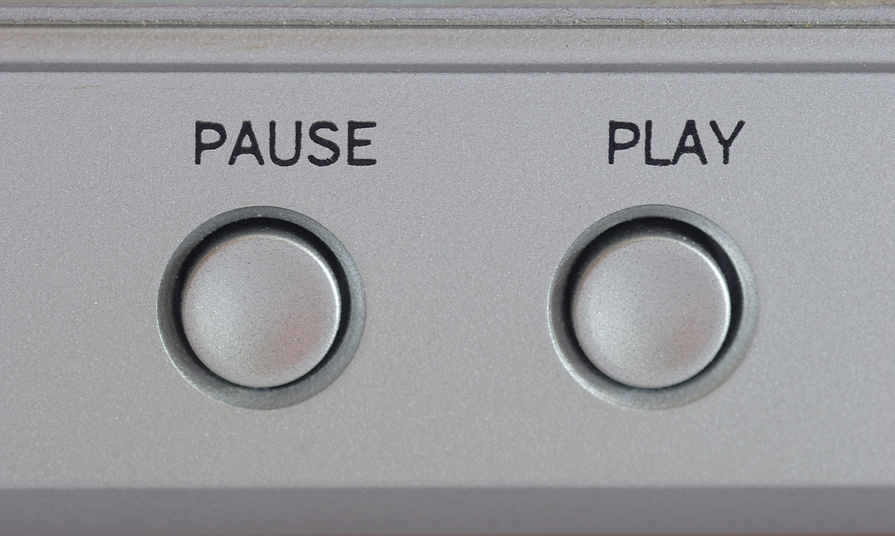
\includegraphics[width=\linewidth]{img/continue.jpg}
\end{frame}

\begin{frame}
  \frametitle{Continuation passing style}
  \begin{itemize}
    \item bla
    \item bla
  \end{itemize}
\end{frame}

\begin{frame}
  \frametitle{Bla bla}
  Bla bla
\end{frame}


\end{document}
